%%%%%%%%%%%%%%%%%%%%%%%%%%%%%%%%%%%%%%%%%
%
% (c) 2019 by Jennifer Laaser
%
% This work is licensed under the Creative Commons Attribution-NonCommercial-ShareAlike 4.0 International License. To view a copy of this license, visit http://creativecommons.org/licenses/by-nc-sa/4.0/ or send a letter to Creative Commons, PO Box 1866, Mountain View, CA 94042, USA.
%
% The current source for these materials is accessible on Github: https://github.com/jlaaser/pogil-polymers
%
%%%%%%%%%%%%%%%%%%%%%%%%%%%%%%%%%%%%%%%%%

\renewcommand{\figpath}{content/polymphys/solution-thermo/phase-diagrams/figs}
\renewcommand{\labelbase}{phase-diagrams}

\begin{activity}{Phase Diagrams of Polymer Solutions}

\begin{instructornotes}

	This activity introduces students to key concepts related to phase diagrams of polymer solutions.
	
	After completing this activity, students will be able to:
			\begin{enumerate}
				\item ...
			\end{enumerate}
	This activity will prepare students for ...
			
	\subsection*{Activity summary:}
	\begin{itemize}
		\item \textbf{Activity type:} Learning Cycle
		\item \textbf{Content goals:} Phase diagrams of polymer solutions
		\item \textbf{Process goals:} %https://pogil.org/uploads/attachments/cj54b5yts006cklx4hh758htf-process-skills-official-pogil-list-2015-original.pdf
			written communication, critical thinking, information processing
		\item \textbf{Duration:} TBD
		\item \textbf{Instructor preparation required:} none beyond knowledge of relevant content
		\item \textbf{Related textbook chapters:}
			\begin{itemize}
				\item \emph{Polymer Chemistry} (Hiemenz \& Lodge): sections XX \& YY
			\end{itemize}
	\end{itemize}

\end{instructornotes}

	%\textbf{Focus question:} Put a central question for the students to consider through this exercise here.


\begin{model}[From Free Energy Curves to Phase Diagrams]
\label{\labelbase:mdl:spinodalbinodal}

	Schematic free energy curves for solutions of polymers with the same degree of polymerization, $N$, but different values of $\chi$, are shown below:
	
	\centerline{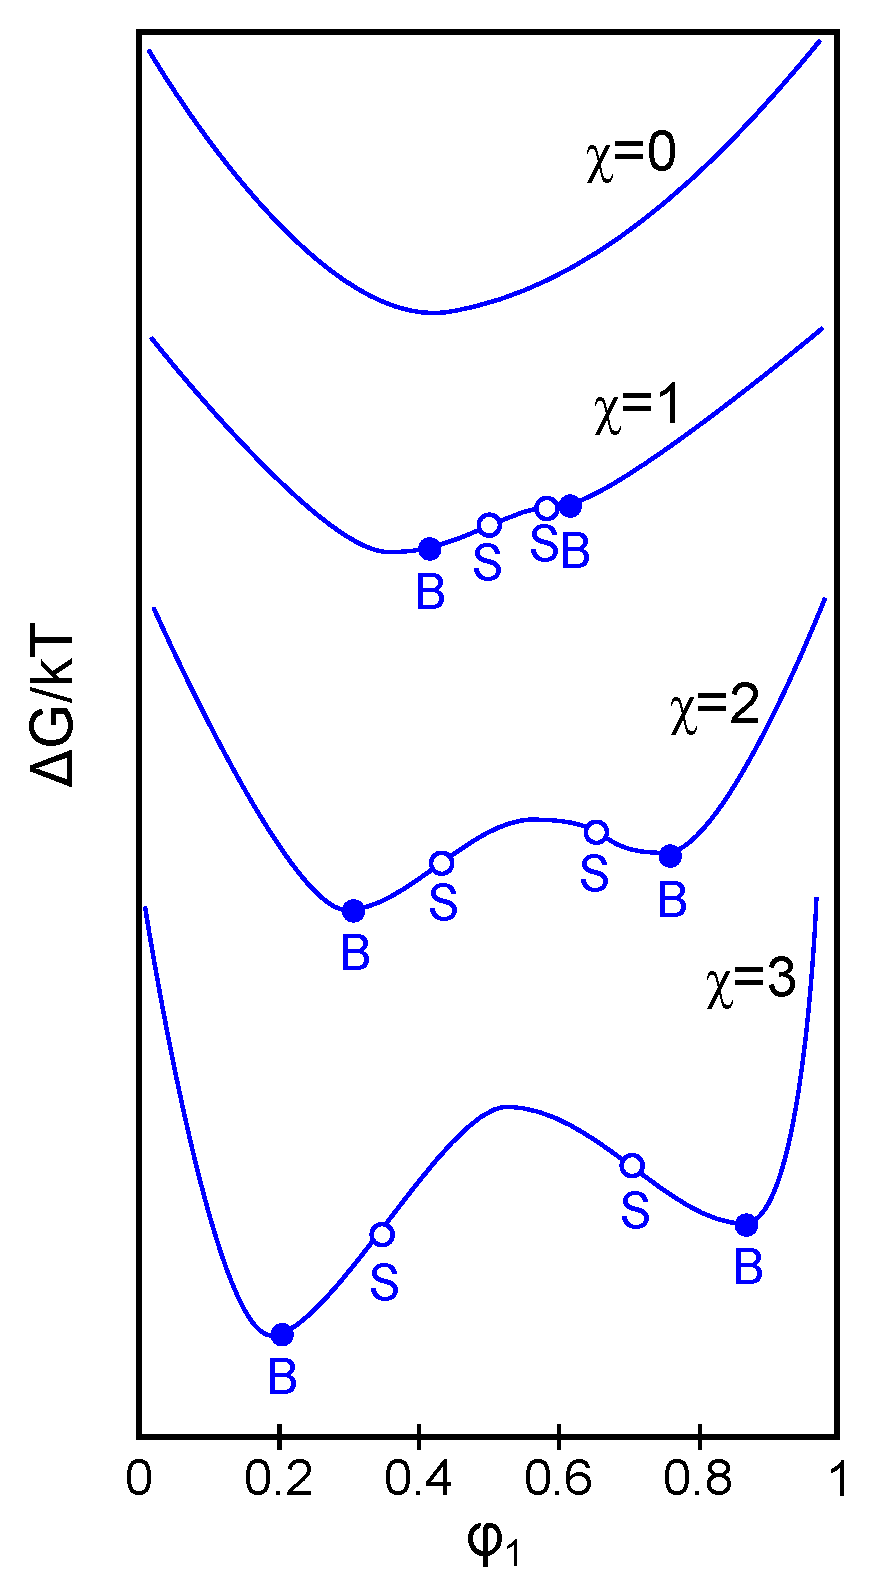
\includegraphics[width=0.4\textwidth]{\figpath/model1-varychi}}
	
	The spinodal (S) and binodal (B) points are marked on the plots where appropriate.
\end{model}

\begin{ctqs}

	\question For which value(s) of $\chi$ will the polymer mixtures...
	
		\begin{enumerate}
			\item ... always form a homogeneous, single-phase solution?
				
				\begin{solution}[0.75in]
				\end{solution}
			
			\item ... phase separate, for some values of $\phi_1$?
				
				\begin{solution}[0.75in]
				\end{solution}
				
		\end{enumerate}
	
	\question Plot the locations of the spinodal and binodal points for each value of $\chi$ on the following axes.  When you have plotted all of the points, draw a smooth curve connecting all of the binodal points, and a second curve connecting all of the spinodal points.
	
		\centerline{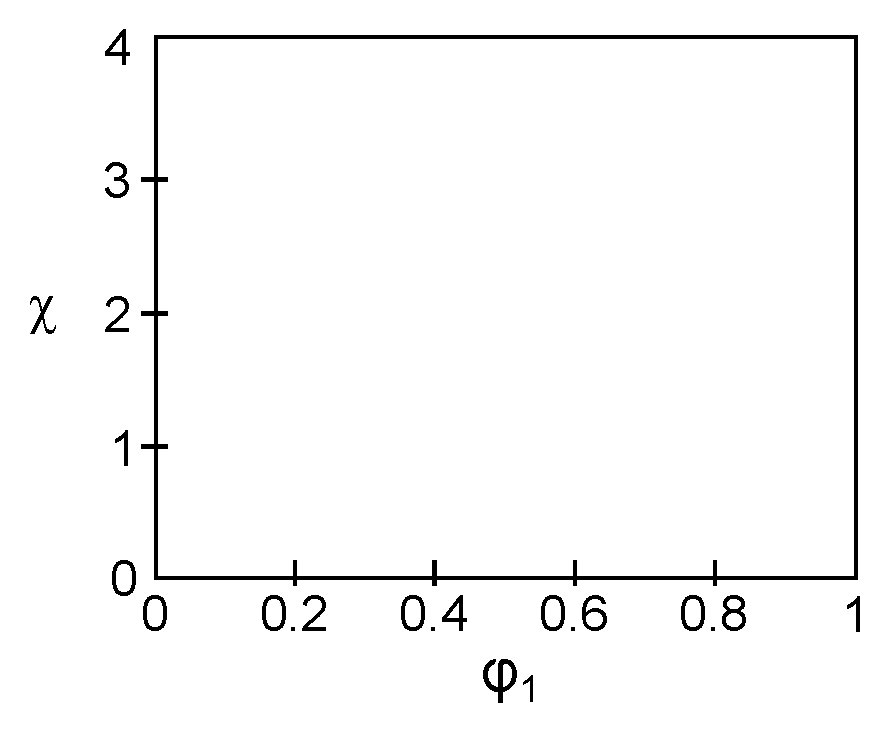
\includegraphics[width=0.4\textwidth]{\figpath/model1-phasediagramchi}}
		
	\question On your plot, label the region in which you expect to always get a one-phase mixture as ``1$\Phi$'', the region in which you expect to always get a two-phase mixture as ``2$\Phi$'', and the region in which you expect to get a metastable one-phase mixture as ``MS''.
		
\end{ctqs}


\begin{infobox}
	For a given polymer/solvent pair, the interaction parameter, $\chi$, generally varies with temperature as
	\begin{equation*}
		\chi = \frac{\alpha}{T} + \beta
	\end{equation*}
\end{infobox}


\begin{ctqs}

	\question Re-plot your curves from the previous question with temperature on the y axis.  For the purposes of this problem, assume that this mixture has $\alpha=200$~K and $\beta=0$.
		\label{\labelbase:ctq:plotT}
	
		\centerline{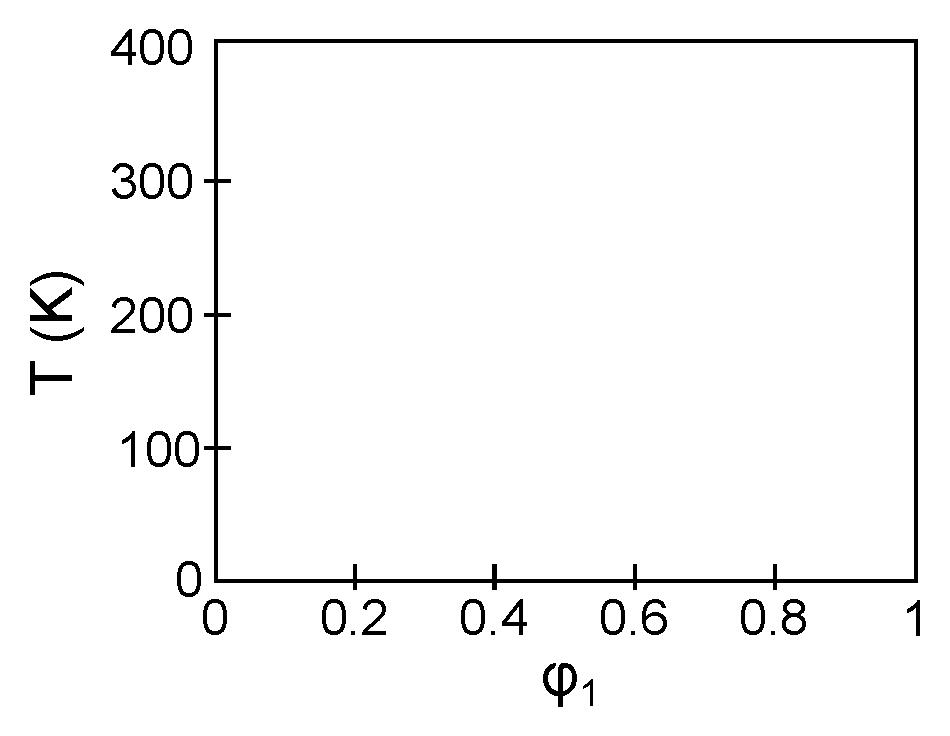
\includegraphics[width=0.45\textwidth]{\figpath/model1-phasediagramT}}
		
	\question On your plot, label the region in which you expect to always get a single-phase mixture as ``1$\Phi$'', the region in which you expect to always get a two-phase mixture as ``2$\Phi$'', and the region in which you expect to get a metastable mixture as ``MS''.
		
		
\end{ctqs}


\begin{infobox}

	The \emph{critical temperature} of a polymer solution, $T_c$, is the temperature above which the mixture will \emph{always} form a homogeneous, single-phase solution.

\end{infobox}


\begin{ctqs}
	\question Estimate the critical temperature for the polymer whose phase diagram you drew in question \ref{\labelbase:ctq:plotT}:
	
		\begin{solution}[0.25in]
		
			Most students will guess something around 300~K, but the exact number is not critical for this question.
		
		\end{solution}
		
\end{ctqs}



\begin{model}[Phase Diagrams of Polymer Solutions]
	\label{\labelbase:mdl:Ndependence}

	The spinodal curves for a series of polymers with the same value of $\chi$ but different degrees of polymerization $N$ are shown below:
	
	\centerline{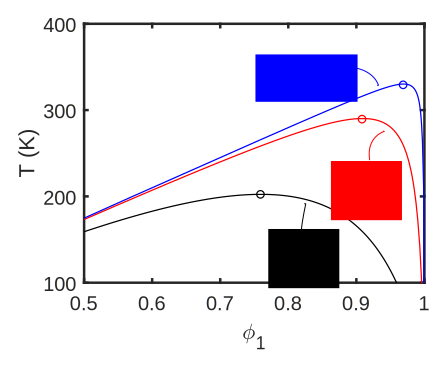
\includegraphics[width=0.5\textwidth]{\figpath/model2-spinodalN-edited}}
	
	The critical point for each curve is indicated with a circle ($\circ$).
	
\end{model}

\begin{ctqs}

	\question Estimate the critical temperature, $T_c$, and the composition at the critical point, $\phi_{1,c}$, for each value of $N$ shown in Model \ref{\labelbase:mdl:Ndependence}:
	
		\begin{center}
			\renewcommand{\arraystretch}{2.5}
			\begin{tabular}{|c|c|c|}
				\hline
				\textbf{N} & \hspace{0.6cm}$\phi_{1,c}$\hspace{0.6cm} & \hspace{0.75cm}$T_c$\hspace{0.75cm} \\\hline
				10 & & \\\hline
				100 & & \\\hline
				1000 & & \\\hline
			\end{tabular}
		\end{center}
		
	\question How do $\phi_{1,c}$ and $T_c$ change as $N$ increases?
	
		\begin{solution}[0.5in]
		\end{solution}
	
	\question What do you expect to happen to the value of $\phi_{1,c}$ in the limit of infinitely long polymer chains ($N\to\infty$)?
	
		\begin{solution}[0.5in]
		\end{solution}
		
	\question What do you expect to happen to the value of $T_c$ in the limit of infinitely long polymer chains ($N\to\infty$)?
	
		\begin{solution}[0.5in]
		\end{solution}

\end{ctqs}


\begin{infobox}
\label{\labelbase:infobox:critpt}
	
	The critical point occurs when the spinodal (and binodal) points converge.  Mathematically, the spinodal points occur when the second-derivative of the free energy is zero:
	\begin{equation*}
		\frac{d^2\Delta G}{d\phi_1^2} = 0
	\end{equation*}
	When the two spinodal points are on top of each other, the \emph{third} derivative of the free energy must also be zero; thus the critical point occurs when 
	\begin{equation*}
		\frac{d^3\Delta G}{d\phi_1^3} = 0
	\end{equation*}
	
	Applying these two conditions (see Exercise \ref{\labelbase:exc:critpt}), we find that the composition at the critical point is
	\begin{equation*}
		\phi_{1,c} = \frac{\sqrt{N}}{1+\sqrt{N}}
	\end{equation*}
	and the interaction parameter at the critical point is
	\begin{equation*}
		\chi_c = \frac{1}{2}\left(\frac{1}{N} + \frac{2}{\sqrt{N}} + 1\right)
	\end{equation*}
	
\end{infobox}



\begin{ctqs}
	
	\question What happens to the value of $\chi_c$ when the chains are only a single monomer ($N=1$)?
	
		\begin{solution}[0.75in]
		\end{solution}
	
	\question What happens to the value of $\chi_c$ when the chains become infinitely long ($N\to\infty$)?	
	
		\begin{solution}[0.75in]
		\end{solution}
	
	\question Based on your answers to the previous questions, critique or defend the following statement:
	
		\emph{``When $\chi > 0.5$, a polymer solution will always phase separate.'' }
	
		\begin{solution}[2.5in]
		\end{solution}

\end{ctqs}


\begin{infobox}
	
	The \emph{theta temperature} of a polymer solution is the temperature at which $\chi=0.5$.
	
\end{infobox}


\begin{ctqs}

	\question Propose a method that you could use to find the theta temperature of a polymer/solvent mixture from phase diagrams such as those shown in Model \ref{\labelbase:mdl:Ndependence}.
	
		\begin{solution}[1.5in]
		\end{solution} 

	\question Using your method, estimate the theta temperature for the polymer shown in Model \ref{\labelbase:mdl:Ndependence}.
	
		\begin{solution}[0.5in]
		\end{solution} 

\end{ctqs}



\begin{exercises}

	\exercise Derive the expressions for $\phi_{1,c}$ and $\chi_c$ given in the activity by doing the following:
		\label{\labelbase:exc:critpt}
	
		\begin{enumerate}
	
			\item First, show that the third derivative of the Flory-Huggins expression for the free energy of a polymer solution is
				\begin{equation*}
					\frac{d^3\Delta G}{d\phi_1^3} = \frac{-1}{\phi_1^2} + \frac{1}{N}\frac{1}{(1-\phi_1)^2}
				\end{equation*}
		
				Then set this expression equal to zero and solve for $\phi_{1,c}$, the composition at the critical point.
		
			\item Second, show that the second derivative of the Flory-Huggins expression for the free energy of a polymer solution is
	
				\begin{equation*}
					\frac{d^2\Delta G}{d\phi_1^2} = -2\chi + \frac{1}{\phi_1} + \frac{1}{N}\frac{1}{1-\phi_1}
				\end{equation*}
		
				Set this expression equal to zero and solve for $\chi$ in terms of $\phi_1$.
				
			\item Finally, substitute in your expression for $\phi_{1,c}$ to find $\chi_c$, the interaction parameter at the critical point, and verify that it is consistent with the equation given on page \pageref{\labelbase:infobox:critpt}.
				
		\end{enumerate}
		
	\exercise Do the following for a polymer solution for which $\chi = \alpha/T$:
		
		\begin{enumerate}
			\item Find an expression for the critical temperature, $T_c$, in terms of the degree of polymerization, $N$.
			\item Find an expression for the theta temperature  in terms of $\alpha$.
		\end{enumerate}
		
	\exercise For the polymer solution whose spinodal curve is shown below,
	
		\centerline{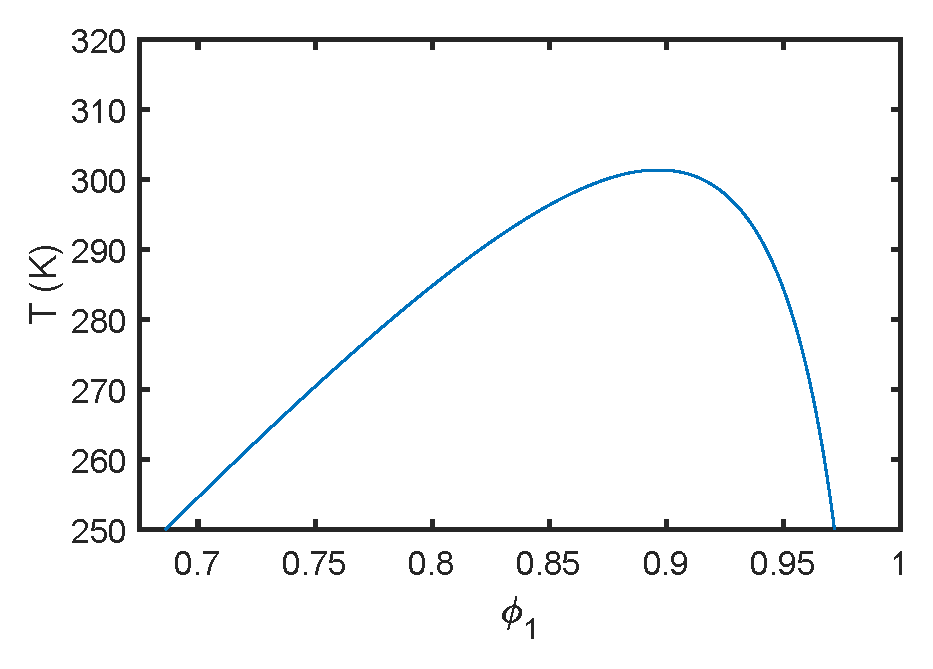
\includegraphics[width=0.5\textwidth]{\figpath/exercise-samplespinodal}}
	
		\begin{enumerate}
			\item Estimate the degree of polymerization of the polymer.
				
				\emph{Hint: start by finding the composition at the critical point, $\phi_{1,c}$.}
			
				\begin{solution}\instructordisplay{
					Correct answer: 75
				}\end{solution}
				
			\item Estimate the interaction parameter, $\chi$, for this polymer mixture.
			
			\item Finally, estimate the theta temperature for this polymer system, assuming that $\chi$ obeys the relationship $\chi = \frac{\alpha}{T}$.
			
				\begin{solution}\instructordisplay{
					Correct answer: 375 K
				}\end{solution}
			
		\end{enumerate}
		
	\exercise What do you expect would happen if you prepared a polymer solution at a very high temperature and then rapidly decreased the temperature of the mixture?
		
\end{exercises}
	
\end{activity}